\chapter{Design and Implementation}\label{chapter:design}

 

\TODO{Wan: It would be good to precede this section with a paragraph on your research aims and approach, so the gist of Sections 1.1 and 1.2. Now you suddenly transition from a general description of Web caching to a technical exposition on cache simulators.}

This chapter tackles the design and implementation of the core components that make up this work's experiment, described in detail in \Cref{chapter:experimental-setup}. As discussed in \Cref{sec: research_q}, this research aims to study the performance of SIEVE against different cache eviction primitives to better assess its competitiveness with workloads that follow Zipf-like distributions. To achieve this goal, we first had to select a suitable cache simulator that was easily extendable with additional algorithm implementations and allowed specifying a workload to run. This choice consequently had an impact on the implementation of the cache eviction algorithms, which were heavily reliant on the framework's structure. Lastly, synthetic workloads following Zipf-like distributions had to be generated to test each algorithm's miss ratio performance when running each cache simulation. 

The approach taken above reveals the three core components necessary in our approach, each of which is further discussed in the following sections: (1) the cache simulator, (2) the eviction algorithms,  and (3) the generated workloads used.

% #############################################################

\section{Cache Simulator}\label{sec: cache-simulations}

\outline{What simulation library is used and why?}

The building and execution of cache simulations was performed using the cache simulator provided by \keyword{libCacheSim}\footnote{GitHub for libCacheSim library: \url{https://github.com/1a1a11a/libCacheSim}}, a high-performance open-source library specifically designed for cache simulation and trace analysis. This tool was chosen because of its simple extensibility of new algorithms, the ability to specify a workload for a single simulation run, and support for various workload formats (including CSV, BIN, TXT, VSCSI). The libCacheSim library's strength lies in its detailed documentation on how to extend the framework with eviction algorithms or trace readers\footnote{Markdown file describing extendability of libCacheSim: \url{https://github.com/1a1a11a/libCacheSim/blob/develop/doc/advanced_lib_extend.md}}.


\subsection{Setup Issues with libCacheSim}\label{sec:setup-issues}

It is notable that the open-source libCacheSim library, written in C/C++, has been developed primarily for Ubuntu 22.04 systems reliant on GCC (GNU Compiler Collection) for compilation. Due to this, there were many compatibility issues when setting up the library on the device used for development: an Apple MacBook Pro M1 reliant on the Clang compiler. 

As part of this work's effort and contribution to the open-source project, many of these issues have been addressed, and GitHub pull requests have been made to improve the open-source project's cross-compatibility. \Cref{PRs} presents a summary of all pull requests made over the course of the project.

Most issues were caused by an unsuccessful compilation on the macOS device (addressed by PR \href{https://github.com/1a1a11a/libCacheSim/pull/183}{\#183}). A major cause of this incompatibility stems from differences in compiler strictness (GCC vs. Clang). Clang is known for being very strict and pedantic with its warnings, especially concerning potential portability issues or undefined behavior\footnote{Clang Compiler's User Manual: \url{https://clang.llvm.org/docs/UsersManual.html\#diagnostics}}, causing many warnings silenced by GCC to be flagged as errors on Clang.

An interesting compilation issue is related to \keyword{format specifier mismatches}. The libCacheSim codebase contains \code{printf} statements for logging various details, many of which use format specifiers (i.e. \code{\%ld}, \code{\%lld}, \code{\%lu}, \code{\%llu}). Variables of certain types use different format specifiers on different platforms. For example, variables of type \code{int64\_t} (signed 64-bit integer) use the \code{\%ld} format specifier on Ubuntu/Linux (with GCC) while \code{\%lld} is needed as a format specifier of the same type on macOS (with Clang). 

\begin{description}[style=unboxed, leftmargin=0cm]
    \item[Naive solution] A naive solution to this compatibility issue could be to use different format specifiers depending on the system's operating system and compiler. This could be done by wrapping \code{printf} statements containing \enquote{problematic} format specifiers in conditional preprocessor macros (i.e. \code{\#ifdef}, \code{\#if defined}, or \code{\#if}). However, this method adds conditional compilation complexity and makes maintenance so much more difficult. 
    \item[Improved solution] A cleaner, more optimal, and fool-proof solution to ensure cross-compatibility is the use of special format macros that expand to the correct format specifier depending on the compilation platform. In the case of the \code{int64\_t} type, which requires format specifier \code{\%ld} on Ubuntu/GCC but \code{\%lld} on macOS/Clang, the \code{PRId64} macro can be used as a portable solution to the format specifier mismatch. The \code{PRId64} macro, defined in the \code{<inttypes.h>} header, is part of a family of macros known as format string macros for fixed-width integers introduced in the C99 standard \footnote{Fixed width integer types (since C99): \url{https://en.cppreference.com/w/c/types/integer}} to address these kinds of portability issues.
\end{description}

This specific issue concerns the non-portable use of format specifiers across platforms, but many different kinds of compilation issues were tackled (see \Cref{PRs}). More details on the issue and fix of format specifier mismatches can be found in the description of the PR \href{https://github.com/1a1a11a/libCacheSim/pull/183}{\#183} itself.

\outline{Describe setup process}




\section{Cache Eviction Algorithms}\label{sec: cache-eviction-algs}

To support the proper execution of a cache eviction algorithm, the libCacheSim simulator requires the implementation of eight methods for a newly added cache eviction algorithm, given by \Cref{code: cache-functions}.

\lstset{style=CStyle}

\begin{lstlisting}[language=C, caption=Functions required for cache eviction algorithms in libCacheSim, label=code: cache-functions]
cache_t *init(const common_cache_params_t ccache_params, const char *cache_specific_params);

void free(cache_t *cache);

bool get(cache_t *cache, const request_t *req);

cache_obj_t *find(cache_t *cache, const request_t *req, const bool update_cache);

cache_obj_t *insert(cache_t *cache, const request_t *req);

cache_obj_t *to_evict(cache_t *cache, const request_t *req);

void evict(cache_t *cache, const request_t *req);

bool remove(cache_t *cache, const obj_id_t obj_id);
\end{lstlisting}

Seeing as all of these methods use parameters with types specific to the library itself (i.e. \code{common\_\\cache\_params\_t}), it was crucial to study the behavior and usage of these in the framework before implementing specific algorithms.

Some important design and implementation details common to all implemented algorithms are discussed below:

\outline{something about why choosing cache eviction PRIMITIVES}

\begin{description}[style=unboxed, leftmargin=0cm]
    \item[Primitives] Notably, the algorithms chosen for this work are not only cache eviction algorithms, but also primitives. In this way, they can build the base for larger, more complex algorithms. The decision to focus primarily on cache eviction primitives stems from the goal to better understand SIEVE and how it compares to alternatives. Given that primitives are often interchangeable in larger cache policies, grasping the strengths and weaknesses of each allows for more effective development of the more complex systems.
    \item[Data structures] All primitives use a doubly-linked list for the queue with pointers to the head and tail. The main difference in their implementation is the eviction strategy; SIEVE uses an additional hand pointer to an item in the doubly-linked list. Furthermore, the libCacheSim simulator offers a built-in hashtable (\code{struct hashtable}) which stores cached objects by mapping keys to cached data. Our algorithm implementations interact with this data structure to get, insert, and remove items. This struct also supports storing metadata such as eviction age, admission status, or object age for each cached item. Notably, these features are not used in our algorithm implementations due to our assumptions of objects having no expiration.
\end{description}

The following subsections give an overview of each of the cache eviction primitives implemented in this work, namely SIEVE, LRU, and FIFO.

\subsection{SIEVE}

SIEVE was first introduced in \citeauthor{sieve}'s \citeyear{sieve} paper entitled \textit{\citetitle{sieve}} \cite{sieve}. The paper's title already alludes to its goal of competing with long-standing cache eviction primitives such as LRU.

SIEVE's authors report that SIEVE is "an algorithm that is simpler than LRU and provides better than state-of-the-art efficiency and scalability for web cache workloads" \cite{sieve}. Additionally, they state that SIEVE not only has a lower miss ratio than other cache eviction algorithms but also demonstrates impressive results against the more complex state-of-the-art algorithms. The focus of this work was primarily motivated by the promising results of the SIEVE algorithm, as presented in the original paper.

The SIEVE cache algorithm is said to achieve its efficiency through some key properties that distinguish it from other caching strategies. The \keyword{moving hand} is a crucial element that is said to function like "an adaptive filter that removes unpopular objects from the cache" \cite{sieve}. Unlike other algorithms that reorder the list on every access, SIEVE employs \keyword{lazy promotion} on a cache hit by simply setting a flag on the entry, entirely avoiding otherwise expensive manipulation. Additionally, \keyword{quick demotion} of unpopular items occurs when the moving hand encounters an item with its promotion flag (also referred to as the "Boolean visited bit") unset, leading to its immediate eviction. If the flag is set, the hand simply clears it and moves on, giving the recently used item a second chance. According to the authors, this simple mechanism allows SIEVE to achieve a low miss ratio with great scalability \cite{sieve}.


% sieve has some specific properties that are described in the paper which are especially powerful for workloads with zipfian distributions. describe them here.

\outline{SIEVE how it works}

\begin{description}
    \item[Design] 
    
    SIEVE's design requires a FIFO queue and a "hand" pointer that traverses it from tail to head and wraps around back to the tail when the head has been reached. Each item in the queue is associated with a Boolean visited bit, which ultimately determines the eviction of items pointed to by the hand. Initially, all objects in the queue have the visited set to false. Then, there are two cases relevant to eviction, depending on whether the item of a new request is already present in the queue:

    \begin{enumerate}[label=(\arabic*)]
        \item \keyword{Cache hit}: If a newly encountered item is already present in the queue, the only change is to set the visited bit of the request item to true; its position in the queue is unchanged (it does not move to the head of the queue). In this way, the popularity of the object is recorded. Notably, the hand pointer remains stationary, and the size of the queue remains constant.
        \item \keyword{Cache miss}: If a newly encountered item is not yet present in the queue, it is always appended at the head of the queue. In the event that the queue is not yet full, the hand pointer remains stationary. However, in the case of a full queue, the hand pointer moves over any visited objects (from tail to head) and sets their visited status to false until encountering an `unpopular' object (with the visited bit set to false) for eviction. It is notable that the new item does not take the place of the evicted item, but is always appended at the head of the queue. 
    \end{enumerate}
\end{description}

\outline{Example}

\begin{figure}[h!]
    \centering
    \caption{Example of SIEVE algorithm}
    \label{fig:sieve-example}
    \begin{subfigure}[b]{0.3\textwidth}
        \centering        
        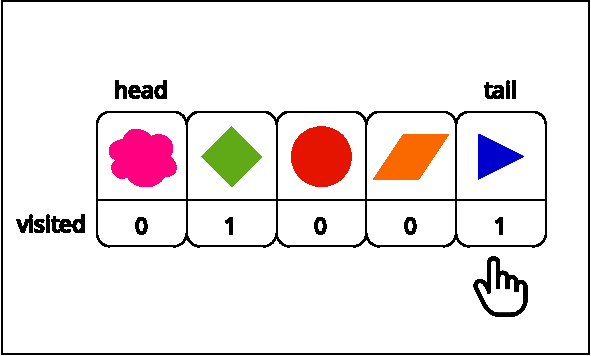
\includegraphics[height=3.1cm]{report/resources/sieve-drawing-1.pdf}
        \caption{Initial cache setup}
        \label{subfig:sieve1}
    \end{subfigure}
    \hfill
    \begin{subfigure}[b]{0.3\textwidth}
        \centering
        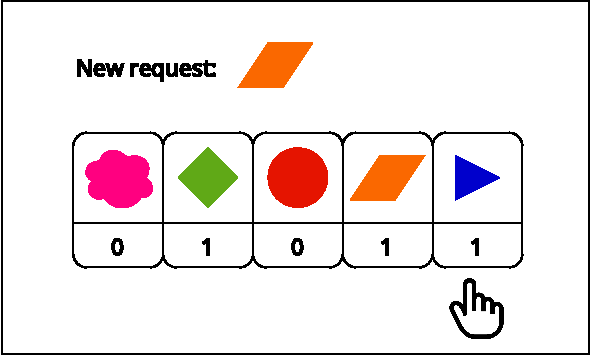
\includegraphics[height=3.1cm]{report/resources/sieve-drawing-2.pdf}
        \caption{Scenario \#1: Cache hit}
        \label{subfig:sieve2}
    \end{subfigure}
    \hfill
    \begin{subfigure}[b]{0.3\textwidth}
        \centering
        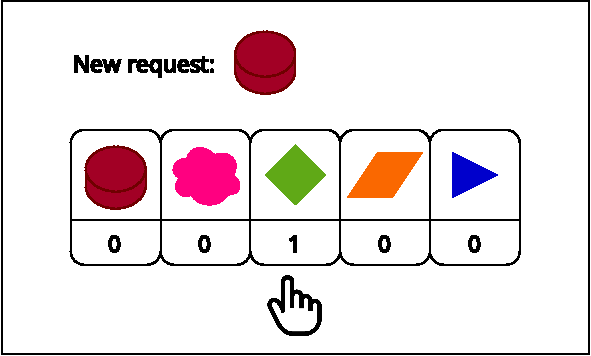
\includegraphics[height=3.1cm]{report/resources/sieve-drawing-3.pdf}
        \caption{Scenario \#2: Cache miss}
        \label{subfig:sieve3}
    \end{subfigure}
\end{figure}

\begin{description}
    \item[Example] To further illustrate the SIEVE caching mechanism, we present an example in \Cref{fig:sieve-example}. Here, we abstract each cache object as a separate shape for the sake of clarity. The initial cache setup is presented in \Cref{subfig:sieve1}, where we can observe that each item in the cache is associated with a different visited status (0 = false, 1 = true) and the queue's head and tail are clearly labeled. In the cache example's initial state, the hand pointer points to the last item of the queue, at the tail ({\color{blue}\textbf{blue triangle}}).

\begin{enumerate}[label=(\arabic*)]
        \item \keyword{Cache hit}:
        In Scenario 1 (\Cref{subfig:sieve2}), the state of the cache is displayed after a cache hit occurs. The newly requested item ({\color{orange}\textbf{orange parallelogram}}) is already present in the cache. Thus, the only change is that the associated item's visited status is set to true ($0\rightarrow1$). There is no displacement of the hand.

        \item \keyword{Cache miss}: 
        After Scenario 1, a cache miss occurs and the cache is left in the state shown by Scenario 2 (\Cref{subfig:sieve3}). The newly requested item ({\color{darkred}\textbf{dark red cylinder}}) is not yet present in the cache, indicating the need for eviction of an item. The hand must traverse the queue from tail to head until it finds its victim (the first item with the visited status set to false). In this case, the victim is the item in the third position ({\color{red}\textbf{red circle}}). Before reaching the victim, the hand passes over two items with their visited status set to true ({\color{blue}\textbf{blue triangle}} and {\color{orange}\textbf{orange parallelogram}}) and toggles these to false before moving on. Once the victim is reached, it is evicted from the queue and the new item is appended to the head of the queue, with its visited state initialised to false.

    \end{enumerate}
\end{description}






\subsection{LRU}

Unlike the newer SIEVE, the LRU (Least Recently Used) replacement policy is foundational to cache systems, having been studied in several early computer systems of the twentieth century \cite{eval-storage-hierarchies, virtual-storage-study}.

\begin{description}
    \item[Design]
    The design of LRU is intuitive and simple, with the principle for cache eviction accurately summarized by its name: "least recently used"; items are evicted in order of recency. Similar to SIEVE, LRU's design uses a queue with head and tail pointers, with new objects always inserted at the head. The notable difference to SIEVE is the lack of a "hand" pointer used to determine the object to evict; instead, the eviction victim always is that which sits at the tail of the queue, signifying that it has been used the least recently. When a newly encountered item is already present in the queue, the item is displaced to the very front of the queue, at its head, effectively signaling its recent use. This displacement of recalled items is different from SIEVE's approach of toggling a visited bit when an item is requested anew (without displacement).
\end{description}


\subsection{FIFO}

Much like the LRU algorithm, the concept of FIFO (First In First Out) is well established, even beyond the realms of cache systems, as a fundamental data structure \cite{lock-free-fifo}. Comparisons between LRU and FIFO in memory systems have also long been discussed \cite{lru-better-than-fifo}. In fact, LRU and FIFO are still used in most caching systems and libraries nowadays \cite{sieve}. For this reason, it is of great interest to study these more foundational algorithms against the newer SIEVE.

\begin{description}
    \item[Design] Similar to LRU, FIFO relies on a single queue with head and tail. New items are added at the head and old items are evicted at the tail: "first in, first out". The crucial difference that makes FIFO a more "primitive" eviction algorithm than LRU is that no displacement of recalled items occurs; if a new item already exists in the queue, its position is left unchanged. In this way, there is no inherent principle that makes some items live longer in the queue than others; all items are given equal priority. This differs from both SIEVE and LRU, which aim to retain popular items in the queue when recalled.
\end{description}


\section{Workloads}\label{sec: workloads}

Web workloads have been widely observed to follow Zipfian distributions, as discussed in \Cref{bkg: zipfian-distributions}. For this reason, this work aims to evaluate algorithms on Zipf-like distributions to simulate the kind of web traffic observed in real life. Due to different skewness parameters being reported across previous research, a range of different $\alpha$ values is tested in this paper. Additionally, the working set sizes used are inspired by those reported across varying open-source and proprietary production datasets in \citeauthor{sieve}'s paper \cite{sieve}, which range from 2\% to 33\% of unique items. More details on the specific parameter values used and the generation of Zipf-like workloads are discussed in \Cref{subsec: synthetic-data-generation}.

% synthetic data
% zipf
% used relative measurements to make it scalable in some sense
